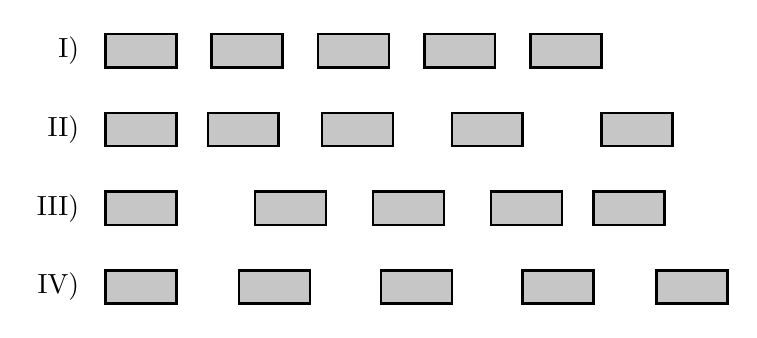
\begin{tikzpicture}[line width=0.9pt]
  \def\blk#1#2{\fill[gray!45] (#1,#2) rectangle ++(0.9,0.42);
    \draw (#1,#2) rectangle ++(0.9,0.42);}
  % Row I : equal spacing
  \node[left] at (-0.2,3.0) {I)};
  \foreach \x in {0,1.35,2.7,4.05,5.4}{\blk{\x}{2.79}}
  % Row II : slowly increasing spacing
  \node[left] at (-0.2,2.0) {II)};
  \foreach \x in {0,1.3,2.75,4.4,6.3}{\blk{\x}{1.79}}
  % Row III : more increasing
  \node[left] at (-0.2,1.0) {III)};
  \foreach \x in {0,1.9,3.4,4.9,6.2}{\blk{\x}{0.79}}
  % Row IV : largest spread
  \node[left] at (-0.2,0.0) {IV)};
  \foreach \x in {0,1.7,3.5,5.3,7.0}{\blk{\x}{-0.21}}
\end{tikzpicture}
